\section{NHIỆT DUNG RIÊNG}
\subsection{LÝ THUYẾT TRỌNG TÂM}
\begin{tomtat}
	\subsubsection{Nhiệt dung riêng}
	\begin{dn}
		Nhiệt dung riêng của một chất là nhiệt lượng cần cung cấp để nhiệt độ của $\SI{1}{\kilogram}$ chất đó tăng thêm $\SI{1}{\kelvin}$.
	\end{dn}
	Đơn vị đo của nhiệt dung riêng trong hệ SI là $\si{\joule/\left(\kilogram\cdot\kelvin\right)}$, nhiệt dung riêng kí hiệu là $c$.
	\subsubsection{Nhiệt lượng trao đổi để khối chất thay đổi nhiệt độ}
	\begin{boxdn}
		Nhiệt lượng trao đổi (toả ra hay nhận vào) để khối chất thay đổi nhiệt độ từ $T_1$ đến nhiệt độ $T_2$:
		$$Q=mc\Delta T$$
	\end{boxdn}
	với:
	\begin{itemize}
		\item $Q$: nhiệt lượng trao đổi, đơn vị trong hệ SI là $\si{\joule}$;
		\item $m$: khối lượng, đơn vị trong hệ SI là $\si{\kilogram}$;
		\item $c$: nhiệt dung riêng của chất tạo nên vật, đơn vị trong hệ SI là $\si{\joule/\left(\kilogram\cdot\kelvin\right)}$;
		\item $\Delta T=T_2-T_1$: độ biến thiên nhiệt độ, đơn vị trong hệ SI là $\si{\kelvin}$.
	\end{itemize}
	\subsubsection{Trạng thái cân bằng nhiệt của hệ nhiệt động}
	\begin{boxdn}
		Hệ nhiệt động đạt trạng thái cân bằng nhiệt khi tổng nhiệt lượng trao đổi trong hệ bằng 0:
		$$\sum Q=Q_1+Q_2+\dots+Q_n=0.$$
	\end{boxdn}
\end{tomtat}
\subsection{VÍ DỤ MINH HOẠ}
\begin{dang}{Xác định nhiệt lượng trao đổi để khối chất thay đổi nhiệt độ}
	\end{dang}
\begin{vd}
Một thùng đựng $\SI{20}{\ell}$ nước ở nhiệt độ $\SI{20}{\celsius}$. Cho khối lượng riêng của nước là $\SI{1000}{\kilogram\cdot\meter^{-3}}$, nhiệt dung riêng của nước $c=\SI{4200}{\joule/\left(\kilogram\cdot\kelvin\right)}$.
			\begin{enumerate}[label=\alph*)]
				\item Tính nhiệt lượng cần truyền cho nước trong thùng để nhiệt độ của nó tăng lên tới $\SI{70}{\celsius}$.
				\item Tính thời gian truyền nhiệt lượng cần thiết nếu dùng một thiết bị điện có công suất $\SI{2.5}{\kilo\watt}$ để đun lượng nước trên. Biết chỉ có $\SI{80}{\percent}$ điện năng tiêu thụ được dùng để làm nóng nước.
			\end{enumerate}
	\loigiai{
				\begin{enumerate}[label=\alph*)]
					\item Khối lượng của $\SI{20}{\ell}$ nước:
					$$m=\rho V=\left(\SI{1000}{\kilogram\cdot\meter^{-3}}\right)\cdot\left(\SI{20E-3}{\meter^{3}}\right)=\SI{20}{\kilogram}.$$
					Nhiệt lượng cần truyền cho nước trong thùng để nhiệt độ của nó tăng lên tới $\SI{70}{\celsius}$:
					$$Q=mc\Delta t=\left(\SI{20}{\kilogram}\right)\cdot\left[\SI{4200}{\joule/\left(\kilogram\cdot\kelvin\right)}\right]\cdot\left(\SI{50}{\kelvin}\right)=\SI{42E5}{\joule}.$$
					\item Năng lượng thiết bị điện tiêu thụ để truyền được nhiệt lượng cần thiết đun nóng nước đến $\SI{70}{\celsius}$:
					$$W=\dfrac{Q}{H}=\SI{52.5E5}{\joule}.$$
					Thời gian đun nước:
					$$t=\dfrac{W}{\calP}=\dfrac{\SI{52.5E5}{\joule}}{\SI{2.5E3}{\watt}}=\SI{2100}{\second}=\SI{35}{\minute}.$$
				\end{enumerate}}
		
\end{vd}
\begin{vd}
	Để làm nguội một sản phẩm bằng đồng có khối lượng $\SI{50}{\gram}$ đã bị nung nóng, người thợ thủ công thả nó vào một bình nhiệt lượng kế đựng $\SI{400}{\gram}$ nước ở $\SI{20}{\celsius}$ từ độ cao cách mặt nước trong bình $\SI{5}{\centi\meter}$. Khi sản phẩm đã nằm yên ở đáy bình và trong bình có cân bằng nhiệt thì nhiệt độ của nước là $\SI{22}{\celsius}$.
	\begin{enumerate}[label=\alph*)]
		\item Dựa vào cơ sở nào để biết nội năng của nước đã biến đổi? Tính độ biến thiên nội năng này.
		\item Nội năng của nước được biến đổi bằng những cách nào? Tính độ biến thiên nội năng của nước gây ra bởi mỗi cách.
		\item Sản phẩm được nung nóng tới nhiệt độ bao nhiêu?
	\end{enumerate}
	Biết độ cao của nước trong bình nhiệt lượng kế là $\SI{20}{\centi\meter}$, nhiệt dung riêng của nước là $\SI{4190}{\joule/\left(\kilogram\cdot\kelvin\right)}$, của đồng là $\SI{380}{\joule/\left(\kilogram\cdot\kelvin\right)}$; lấy $g=\SI{9.81}{\meter/\second^2}$. Bỏ qua sự truyền năng lượng của nước, sản phẩm cho bình nhiệt lượng kế và môi trường xung quanh. Coi lượng nước trong bình không đổi và lực đẩy Archimedes là không đáng kể.
	\loigiai{
		Đây là bài toán về sự biến đổi nội năng bằng cả hai cách: nhận công và truyền nhiệt.\\
		\textbf{	Xác định trạng thái ban đầu và cuối của hệ vật:}\\
		Vì bỏ qua mọi sự truyền năng lượng cho nhiệt lượng kế và môi trường xung quanh nên hệ trao đổi năng lượng chỉ có nước trong nhiệt lượng kế và sản phẩm.
		\begin{itemize}
			\item Trạng thái đầu: Nước ở nhiệt độ $t_1=\SI{20}{\celsius}$; sản phẩm ở độ cao $h_1=\SI{0.25}{\meter}$ so với đáy bình và nhiệt độ $\xsi{t}{\celsius}$.
			\item Trạng thái cuối: Nước ở nhiệt độ $t_2=\SI{22}{\celsius}$; sản phẩm ở độ cao $h_2=\SI{0}{\meter}$ và nhiệt độ $\SI{22}{\celsius}$.
		\end{itemize}
		\begin{enumerate}[label=\alph*)]
			\item Dựa vào sự tăng nhiệt độ của nước mà biết nội năng của nước tăng.\\
			Do nước muốn tăng nhiệt độ $\Delta t_n=t_2-t_1$ thì phải nhận thêm nhiệt lượng $Q_n=m_nc_n\Delta t_n=\left(\SI{0.4}{\kilogram}\right)\cdot\left[\SI{4190}{\joule/\left(\kilogram\cdot\kelvin\right)}\right]\cdot\left(\SI{22}{\celsius}-\SI{20}{\celsius}\right)=\SI{3352}{\joule}$, nên độ tăng nội năng của nước là:
			$$\Delta U=Q_n=\SI{3352}{\joule}.$$
			\item Nội năng của nước tăng lên bằng hai cách là nhận công của sản phẩm khi rơi và nhận nhiệt của sản phẩm truyền cho.\\
			Sản phẩm rơi vào nước bị nước cản nên phải thực hiện công để chống lại sức cản của nước. Do bỏ qua tác dụng của lực đẩy Archimedes, nên công do sản phẩm thực hiện bằng công trọng lực của sản phẩm:
			$$A=W_\text{t1}-W_\text{t2}=mg\left(h_1-h_2\right)=\left(\SI{0.05}{\kilogram}\right)\cdot\left(\SI{9.81}{\meter/\second^2}\right)\cdot\left(\SI{0.25}{\meter}-\SI{0}{\meter}\right)\approx\SI{0.12}{\joule}.$$
			Độ tăng nội năng của nước do nhận được công là $\SI{0.12}{\joule}$.\\
			Sản phẩm bị nung nóng nên khi rơi vào nước nó truyền nhiệt cho nước. Theo định luật I nhiệt động lực học, ta tính được nhiệt lượng do sản phẩm toả ra:
			$$Q=\Delta U-A=\SI{3352}{\joule}-\SI{0.12}{\joule}=\SI{3351.88}{\joule}.$$
			Độ tăng nội năng của nước do truyền nhiệt là $\SI{3351.88}{\joule}.$
			\item Độ biến thiên nhiệt độ của sản phẩm:
			$$Q_s=m_sc_s\Delta t_s\Rightarrow \Delta t_s=\dfrac{Q_s}{m_sc_s}$$
			Vì nhiệt lượng do nước nhận được bằng nhiệt lượng do sản phẩm toả ra nên $Q_s=-Q=-\SI{3351.88}{\joule}.$
			\begin{eqnarray*}
				&	\Rightarrow& t_s-t_0=\dfrac{-\SI{3351.88}{\joule}}{\left(\SI{0.05}{\kilogram}\right)\cdot\left(\SI{380}{\joule/\kilogram\cdot\kelvin}\right)}\approx-\SI{176.41}{\celsius}
				\\
				&\Rightarrow& t_0=t_s+\SI{176.41}{\celsius}=\SI{198.41}{\celsius}.
			\end{eqnarray*}
	\end{enumerate}}
\end{vd}
\begin{dang}{Vận dụng phương trình cân bằng nhiệt}
	\end{dang}
\begin{vd}
		Một bác thợ rèn nhúng một con dao rựa bằng thép có khối lượng $\SI{1.1}{\kilogram}$ ở nhiệt độ $\SI{850}{\celsius}$ vào trong bể nước lạnh để làm tăng độ cứng của lưỡi dao. Nước trong bể có thể tích $\SI{200}{\ell}$ và có nhiệt độ bằng nhiệt độ ngoài trời là $\SI{27}{\celsius}$. Xác định nhiệt độ của nước khi có sự cân bằng nhiệt. Bỏ qua sự truyền nhiệt cho thành bể, môi trường bên ngoài và bỏ qua quá trình nước hoá hơi khi vừa tiếp xúc với rựa. Biết nhiệt dung riêng của thép là $\SI{460}{\joule/\left(\kilogram\cdot\kelvin\right)}$; của nước là $\SI{4180}{\joule/\left(\kilogram\cdot\kelvin\right)}$.
\loigiai{
			Gọi $t_\text{cb}$ là nhiệt độ của nước khi có sự cân bằng nhiệt.\\
			Hệ đạt trạng thái cân bằng nhiệt khi tổng nhiệt lượng trao đổi trong hệ bằng 0:
			\begin{eqnarray*}
				&&	Q_\text{rựa}+Q_\text{nước}=0\\
				&\Leftrightarrow&	m_\text{t}c_\text{t}\left(t_\text{cb}-t_\text{t}\right)+m_\text{n}c_\text{n}\left(t_\text{cb}-t_\text{n}\right)=0\\
				&\Rightarrow& t_\text{cb}=\dfrac{m_\text{n}c_\text{n}t_\text{n}+m_\text{t}c_\text{t}t_\text{t}}{m_\text{n}c_\text{n}+m_\text{t}c_\text{t}}\approx\SI{27.5}{\celsius}.
			\end{eqnarray*}
		}
\end{vd}
	
\begin{vd}
Một bình nhiệt lượng kế bằng nhôm có khối lượng $m_1=\SI{200}{\gram}$ chứa $m_2=\SI{400}{\gram}$ nước ở nhiệt độ $t_1=\SI{20}{\celsius}$. Đổ thêm vào bình một khối lượng nước $m$ ở nhiệt độ $t_2=\SI{5}{\celsius}$. Khi cân bằng nhiệt thì nhiệt độ của nước trong bình là $t=\SI{10}{\celsius}$. Cho biết nhiệt dung riêng của nhôm là $c_1=\SI{880}{\joule/\left(\kilogram\cdot\kelvin\right)}$, của nước là $c_2=\SI{4200}{\joule/\left(\kilogram\cdot\kelvin\right)}$. Bỏ qua sự trao đổi nhiệt với môi trường. Xác định giá trị của $m$.
\loigiai{Khi hệ đạt trạng thái cân bằng nhiệt thì tổng nhiệt lượng trao đổi của hệ bằng 0:
			$$mc_2\left(t-t_2\right)+m_1c_1\left(t-t_1\right)+m_2c_2\left(t-t_1\right)=0$$
			\begin{eqnarray*}
				\Rightarrow m&=&\dfrac{m_1c_1\left(t-t_1\right)+m_2c_2\left(t-t_1\right)}{c_2\left(t_2-t\right)}\\
				&=&\dfrac{\left\{\left(\SI{0.2}{\kilogram}\right)\cdot\left[\SI{880}{\joule/\left(\kilogram\cdot\kelvin\right)}\right]+\left(\SI{0.4}{\kilogram}\right)\cdot\left[\SI{4200}{\joule/\left(\kilogram\cdot\kelvin\right)}\right]\right\}\cdot\left(\SI{10}{\celsius}-\SI{20}{\celsius}\right)}{\left[\SI{4200}{\joule/\left(\kilogram\cdot\kelvin\right)}\right]\cdot\left(\SI{5}{\celsius}-\SI{10}{\celsius}\right)}\\
				&\approx&\SI{0.88}{\kilogram}.
			\end{eqnarray*}
		}
\end{vd}
\subsection{BÀI TẬP TRẮC NGHIỆM}
\setcounter{ex}{0}
\Opensolutionfile{ans}[ans/G12Y24B4TN]
% ===================================================================
\begin{ex}
	Nhiệt lượng vật trao đổi để thay đổi nhiệt độ phụ thuộc vào
	\choice
	{khối lượng, thể tích và độ thay đổi nhiệt độ của vật}
	{ thể tích, nhiệt độ ban đầu và chất cấu tạo nên vật}
	{\True  khối lượng của vật, chất cấu tạo nên vật và độ thay đổi nhiệt độ của vật}
	{nhiệt độ ban đầu, nhiệt độ lúc sau và áp suất của môi trường}
	\loigiai{ }
	\end{ex}
% ===================================================================
\begin{ex}
	Có 4 bình A, B, C, D đều đựng nước ở cùng một nhiệt độ với thể tích tương ứng là: 1 lít, 2 lít, 3 lít, 4 lít. Sau
	khi dùng các đèn cồn giống hệt nhau để đun các bình này khác nhau. Bình có nhiệt độ thấp nhất là
	\begin{center}
		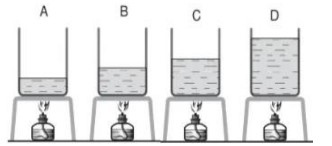
\includegraphics[width=0.4\linewidth]{figs/VN12-Y24-PH-SYL-004P-1}
	\end{center}
	\choice
	{bình A}
	{bình B}
	{bình C}
	{\True bình D}
	\loigiai{}
\end{ex}
% ===================================================================
\begin{ex}
	Chọn phát biểu \textbf{sai}.\\
	Nhiệt dung riêng của một chất 
	\choice
	{là nhiệt lượng cần truyền để $\SI{1}{\kilogram}$ chất đó tăng thêm $\SI{1}{\celsius}$}
	{\True phụ thuộc vào khối lượng riêng của chất đó}
	{phụ thuộc vào bản chất của chất đó}
	{có đơn vị là $\si{\joule/\kilogram\cdot\kelvin}$}
	\loigiai{}
\end{ex}
% ===================================================================
\begin{ex}
Nhiệt độ của vật nào tăng lên nhiều nhất khi ta thả rơi bốn vật dưới đây có cùng khối lượng và từ cùng một độ cao xuống đất? Coi như toàn bộ cơ năng của vật chuyển hoá thành nhiệt năng.
	\choice
	{Vật bằng nhôm, có nhiệt dung riêng là $\SI{880}{\joule/\kilogram\cdot\kelvin}$}
	{Vật bằng đồng, có nhiệt dung riêng là $\SI{380}{\joule/\kilogram\cdot\kelvin}$}
	{\True Vật bằng chì, có nhiệt dung riêng là $\SI{120}{\joule/\kilogram\cdot\kelvin}$}
	{Vật bằng gang, có nhiệt dung riêng là $\SI{5500}{\joule/\kilogram\cdot\kelvin}$}
	\loigiai{$$\Delta t=\dfrac{Q}{mc}.$$
		Vì chì có nhiệt dung riêng nhỏ nhất nên có độ tăng nhiệt độ nhiều nhất}
\end{ex}
% ===================================================================
\begin{ex}
	Tính nhiệt lượng do miếng sắt khối lượng $\SI{2}{\kilogram}$ toả ra khi hạ nhiệt độ từ $\SI{500}{\celsius}$ xuống còn $\SI{40}{\celsius}$. Biết nhiệt dung riêng của sắt là $\SI{478}{\joule/\left(\kilogram\cdot\kelvin\right)}$
	\choice
	{$\SI{219880}{\joule}$}
	{\True $\SI{439760}{\joule}$}
	{$\SI{879520}{\joule}$}
	{$\SI{109940}{\joule}$}
	\loigiai{
		Nhiệt lượng miếng sắt toả ra:
		$$Q=mc\left(t_1-t_2\right)=\SI{439760}{\joule}.$$	
	}
\end{ex}
% ===================================================================
\begin{ex}
	Một viên đạn bằng bạc đang bay với tốc độ $\SI{200}{\meter/\second}$ thì va chạm vào một bức tường gỗ và nằm yên trong bức tường. Nhiệt dung riêng của bạc là $\SI{234}{\joule/\left(\kilogram\cdot\kelvin\right)}$. Nếu coi viên đạn không trao đổi nhiệt với bên ngoài thì nhiệt độ của viên đạn sẽ tăng thêm bao nhiêu độ?
	\choice
	{$\SI{58}{\celsius}$}
	{$\SI{171}{\celsius}$}
	{\True $\SI{85}{\celsius}$}
	{$\SI{250}{\celsius}$}
	\loigiai{
		Áp dụng định luật bảo toàn và chuyển hoá năng lượng:
		$$\dfrac{1}{2}mv^2=mc\Delta t\Rightarrow \Delta t=\dfrac{v^2}{2c}\approx\SI{85}{\celsius}.$$	
	}
\end{ex}
% ===================================================================
\begin{ex}
	Người ta cọ xát hai vật với nhau, nhiệt dung của hai vật là $\SI{800}{\joule/\kelvin}$. Sau 1 phút người ta thấy nhiệt độ của mỗi vật tăng thêm $\SI{30}{\kelvin}$. Công suất trung bình của việc cọ xát bằng
	\choice
	{$\SI{1080}{\watt}$}
	{$\SI{980}{\watt}$}
	{$\SI{480}{\watt}$}
	{\True $\SI{800}{\watt}$}
	\loigiai{	Công suất trung bình của việc cọ xát là
		$$\calP=\dfrac{2c\Delta T}{t}=\SI{800}{\watt}.$$}
\end{ex}
% ===================================================================
\begin{ex}
	Đầu thép của một búa máy có khối lượng $\SI{12}{\kilogram}$ nóng lên thêm $\SI{20}{\celsius}$ sau 1,5 phút hoạt động. Biết rằng  $\SI{40}{\percent}$ cơ năng của búa máy chuyển thành nhiệt năng của đầu búa. Nhiệt dung riêng của thép là $\SI{460}{\joule/\kilogram\cdot\kelvin}$. Công suất của búa gần nhất với giá trị nào sau đây?
	\choice
	{\True $\SI{3}{\kilo\watt}$}
	{$\SI{4}{\kilo\watt}$}
	{$\SI{5}{\kilo\watt}$}
	{$\SI{6}{\kilo\watt}$}
	\loigiai{		Công suất toả nhiệt trên đầu búa:
		$$\calP_\text{hp}=\dfrac{mc\Delta T}{t}\approx\SI{1226.67}{\watt}.$$
		Công suất của búa:
		$$\calP=\dfrac{\calP_\text{hp}}{0,4}\approx\SI{3.066}{\kilo\watt}.$$}
\end{ex}
% ===================================================================
\begin{ex}
	\immini{Quả cầu kim loại được làm bằng chất có nhiệt dung riêng $c=\SI{460}{\joule/\left(\kilogram\cdot\kelvin\right)}$ được treo bởi sợi day có chiều dài $\ell=\SI{46}{\centi\meter}$. Quả cầu được nâng lên đến B rồi thả rơi. Sau khi chạm tường, nó bật lên đến C $\left(\alpha=\SI{60}{\degree}\right)$. Biết rằng $\SI{60}{\percent}$ độ giảm thế năng của quả cầu biến thành nhiệt làm nóng quả cầu. Lấy $g=\SI{10}{\meter/\second^2}$. Độ tăng nhiệt độ của quả cầu là
\choice
{\True $\SI{3E-3}{\celsius}$}
{$\SI{6E-3}{\celsius}$}
{$\SI{1.5E-3}{\celsius}$}
{Không đủ dữ kiện để xác định}	
}{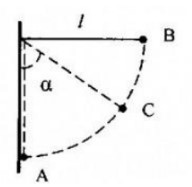
\includegraphics[scale=0.8]{figs/VN12-Y24-PH-SYL-004P-2}
}
	\loigiai{Độ tăng nhiệt độ của quả cầu:
		$$\Delta t=\dfrac{0,6mg\ell\cos\SI{60}{\degree}}{mc}=\dfrac{0,6g\ell\cos\SI{60}{\degree}}{c}=\SI{3E-3}{\celsius}.$$}
\end{ex}
% ===================================================================
\begin{ex}
	Có hai quả cầu bằng chì giống nhau có nhiệt dung riêng là $c$, chuyển động đến va chạm mềm trực diện với tốc độ lần lượt là $v$ và $2v$. Cho rằng toàn bộ cơ năng mất mát trong quá trình va chạm chuyển hoá thành nhiệt năng làm nóng hai quả cầu. Độ tăng nhiệt độ của hai quả cầu là
		\choice
		{\True $\dfrac{9v^2}{8c}$}
		{$\dfrac{7v^2}{8c}$}
		{$\dfrac{9v^2}{7c}$}
		{$\dfrac{11v^2}{7c}$}
	\loigiai{Tốc độ hai quả cầu sau va chạm:
		$$V=\dfrac{2mv-mv}{2m}=0,5v.$$
		Nhiệt lượng toả ra trong quá trình va chạm:
		$$Q=\dfrac{1}{2}mv^2+\dfrac{1}{2}m\left(2v\right)^2-\dfrac{1}{2}\cdot 2mV^2=\dfrac{9}{4}mv^2.$$
		Độ tăng nhiệt độ của hai quả cầu:
		$$\Delta t=\dfrac{Q}{2mc}=\dfrac{9v^2}{8c}.$$}
\end{ex}
% ===================================================================
\begin{ex}
Một lượng nước và một lượng rượu có thể tích bằng nhau, được cung cấp nhiệt lượng tương ứng là $Q_1$ và $Q_2$. Biết khối lượng riêng của nước là $\SI{1000}{\kilogram/\meter^3}$ và của rượu là $\SI{800}{\kilogram/\meter^3}$, nhiệt dung riêng của nước là $\SI{4200}{\joule/\kilogram\cdot\kelvin}$ và của rượu là $\SI{2500}{\joule/\kilogram\cdot\kelvin}$. Để độ tăng nhiệt độ của nước và rượu bằng nhau thì
	\choice
	{$Q_1=Q_2$}
	{$Q_1=1,25Q_2$}
	{$Q_1=1,68Q_2$}
	{\True $Q_1=2,1Q_2$}
	\loigiai{	$$\dfrac{Q_1}{Q_2}=\dfrac{m_1c_1\Delta t}{m_2c_2\Delta t}=\dfrac{D_1c_1}{D_2c_2}=2,1.$$}
\end{ex}
% ===================================================================
\begin{ex}
	Một ấm đồng khối lượng $\SI{300}{\gram}$ chứa 1 lít nước ở nhiệt độ $\SI{15}{\celsius}$. Biết trung bình mỗi giây bếp truyền cho ấm một nhiệt lượng là $\SI{500}{\joule}$. Bỏ qua sự hao phí về nhiệt ra môi trường xung quanh. Lấy nhiệt dung riêng của đồng là $\SI{380}{\joule/\kilogram\cdot\kelvin}$ và của nước là $\SI{4186}{\joule/\kilogram\cdot\kelvin}$. Thời gian đun sôi ấm nước có giá trị gần đúng là
	\choice
	{\True 12 phút}
	{13 phút}
	{14 phút}
	{15 phút}
	\loigiai{Nhiệt lượng nước và ấm cần thu vào để sôi:
		$$Q=\left(m_1c_1+m_2c_2\right)\Delta t=\SI{365500}{\joule}.$$
		Thời gian đun sôi ấm nước:
		$$t=\dfrac{Q}{\SI{500}{\joule/\second}}=\SI{731}{\second}\approx\SI{12}{\text{phút}}.$$}
\end{ex}
% ===================================================================
\begin{ex}
	Người ta muốn pha nước tắm với nhiệt độ $\SI{38}{\celsius}$ thì phải pha bao nhiêu lít nước sôi vào 15 lít nước lạnh ở $\SI{24}{\celsius}$?
	\choice
	{2,5 lít}
	{\True 3,38 lít}
	{4,2 lít}
	{5 lít}
	\loigiai{$$Q_1+Q_2=0\Leftrightarrow V_1\rho c\left(t_\text{cb}-t_1\right)+V_2\rho c\left(t_\text{cb}-t_2\right)=0$$
		$$\Leftrightarrow V_1\left(38-100\right)+15\cdot\left(38-24\right)=0\Rightarrow V_1=\SI{3.38}{\liter}.$$}
\end{ex}
% ===================================================================
\begin{ex}
	Một ấm đun nước bằng nhôm có khối lượng $\SI{400}{\gram}$, chứa 3 lít nước được đun trên bếp. Khi nhận thêm nhiệt lượng $\SI{740}{\kilo\joule}$ thì ấm đạt đến nhiệt độ $\SI{80}{\celsius}$. Biết nhiệt dung riêng của nhôm và nước lần lượt là $c_1=\SI{880}{\joule/\left(\kilogram\cdot\kelvin\right)}$, $c_2=\SI{4190}{\joule/\left(\kilogram\cdot\kelvin\right)}$. Nhiệt độ ban đầu của ấm là
	\choice
	{$\SI{8.15}{\celsius}$}
	{$\SI{8.15}{\kelvin}$}
	{\True $\SI{22.7}{\celsius}$}
	{$\SI{22.7}{\kelvin}$}
	\loigiai{$$Q=\left(m_1c_1+m_2c_2\right)\Delta t\Rightarrow \Delta t=\dfrac{Q}{m_1c_1+m_2c_2}\approx\SI{57.27}{\celsius}.$$
		Nhiệt độ ban đầu của ấm:
		$$t_1=t_2-\Delta t=\SI{22.73}{\celsius}.$$}
\end{ex}
% ===================================================================
\begin{ex}
	Người ta thả một vật rắn khối lượng $m_{1}$ nhiệt độ \SI{150}{\celsius} vào một bình chứa nước có khối lượng $m_{2}$ thì khi cân bằng nhiệt, nhiệt độ của nước tăng từ \SI{10}{\celsius} đến \SI{50}{\celsius}. Gọi $c_{1}, c_{2}$ lần lượt là nhiệt dung riêng của vật rắn và nhiệt dung riêng của nước. Bỏ qua sự hấp thụ nhiệt của bình và môi trường xung quanh. Tỉ số đúng là
	\choice
	{$\dfrac{m_{1} c_{1}}{m_{2} c_{2}}=\dfrac{7}{2}$}
	{$\dfrac{m_{1} c_{1}}{m_{2} c_{2}}=\dfrac{2}{7}$}
	{$\dfrac{m_{1} c_{1}}{m_{2} c_{2}}=\dfrac{5}{2}$}
	{\True $\dfrac{m_{1} c_{1}}{m_{2} c_{2}}=\dfrac{2}{5}$}
	\loigiai{}
\end{ex}
% ===================================================================
\begin{ex}
Thả một miếng thép $\SI{2}{\kilogram}$ đang ở nhiệt độ $\SI{345}{\celsius}$ vào một bình đựng 3 lít nước. Sau khi cân bằng nhiệt, nhiệt độ cuối cùng của nước là $\SI{30}{\celsius}$. Bỏ qua sự trao đổi nhiệt với môi trường. Nhiệt dung riêng của thép và nước lần lượt là $\SI{460}{\joule/\kilogram\cdot\kelvin}$, $\SI{4200}{\joule/\kilogram\cdot\kelvin}$. Nhiệt độ ban đầu của nước là
	\choice
	{\True $\SI{7}{\celsius}$}
	{$\SI{17}{\celsius}$}
	{$\SI{27}{\celsius}$}
	{$\SI{37}{\celsius}$}
	\loigiai{Khi hệ đạt trạng thái cân bằng nhiệt thì tổng nhiệt lượng trao đổi trong hệ bằng 0:
		$$m_1c_1\left(t-t_1\right)+m_2c_2\left(t-t_2\right)=0$$
		$$\Leftrightarrow 2\cdot460\cdot\left(\SI{30}{\celsius}-\SI{345}{\celsius}\right)+3\cdot 4200\left(\SI{30}{\celsius}-t_2\right)=0\Rightarrow t_2=\SI{7}{\celsius}.$$}
\end{ex}

% ===================================================================
\begin{ex}
	Thả một quả cầu bằng nhôm có khối lượng $\SI{0.21}{\kilogram}$ được nung nóng đến $\SI{200}{\celsius}$ vào cốc đựng nước ở $\SI{30}{\celsius}$. Sau một thời gian, nhiệt độ của nước và quả cầu đều bằng $\SI{50}{\celsius}$. Biết nhiệt dung riêng của nhôm là $\SI{880}{\joule/\left(\kilogram\cdot\kelvin\right)}$, nhiệt dung riêng của nước là $\SI{4200}{\joule/\left(\kilogram\cdot\kelvin\right)}$. Khối lượng nước trong cốc là	
	\choice
	{$\SI{3.3}{\kilogram}$}
	{$\SI{7.5}{\kilogram}$}
	{$\SI{0.21}{\kilogram}$}
	{\True $\SI{0.33}{\kilogram}$}
	\loigiai{
		Áp dụng phương trình cân bằng nhiệt:
		$$m_1c_1\left(t_\text{cb}-t_1\right)+m_2c_2\left(t_\text{cb}-t_2\right)=0$$
		$$\Rightarrow m_2=\dfrac{m_1c_1\left(t_\text{cb}-t_1\right)}{c_2\left(t_2-t_\text{cb}\right)}=\SI{0.33}{\kilogram}.$$ }
	
\end{ex}
\textbf{\textit{Sử dụng thông tin sau cho Câu 18, Câu 19 và Câu 20}}\\
\immini{Hình bên là sơ đồ nguyên lí làm mát bằng dầu của một máy biến áp. Lõi từ và các cuộn dây của máy biến áp được ngâm trong bể dầu. Khi lõi từ và các cuộn dây nóng lên thì nhiệt độ của dầu tăng lên. Dầu được lưu thông qua bộ trao đổi nhiệt để làm mát. Biết rằng nhiệt độ của dầu khi bắt đầu đi vào bộ trao đổi nhiệt là \SI{85}{\celsius} và sau khi làm mát là \SI{55}{\celsius}; dầu sử dụng có nhiệt dung riêng là $c=\SI{2000}{\joule/\left(\kilogram\cdot\kelvin\right)}$ và khối lượng riêng là \SI{850}{\kilogram/\meter^3}; tổn thất nhiệt của máy biến áp khi vận hành là \SI{500}{\kilo\watt}.}{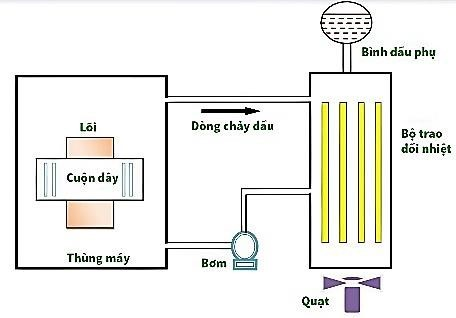
\includegraphics[scale=0.4]{figs/G12Y24B4-5}}
% ===================================================================
\begin{ex}
	Nhiệt lượng tỏa ra khi có 4 lít dầu được làm mát qua bộ trao đổi nhiệt là
	\choice
	{\SI{240}{\kilo\joule}}
	{\SI{240}{\mega\joule}}
	{\SI{204}{\mega\joule}}
	{\True \SI{204}{\kilo\joule}}
	\loigiai{}
\end{ex}
% ===================================================================
\begin{ex}
	Khi dầu đi qua cuộn dây máy biến áp thì nội năng của dầu
	\choice
	{giảm đi}
	{\True tăng lên}
	{không đổi}
	{đạt giá trị tối thiểu}
	\loigiai{}
\end{ex}
% ===================================================================
\begin{ex}
	Giả sử toàn bộ nhiệt lượng tỏa ra trên máy biến áp đều tản ra khi dầu đi qua bộ trao đổi nhiệt. Khối lượng dầu lưu thông qua bộ trao đổi nhiệt trong một phút là bao nhiêu?
	\choice
	{\SI{529}{\kilogram}}
	{\SI{833}{\kilogram}}
	{\SI{5000}{\kilogram}}
	{\True \SI{500}{\kilogram}}
	\loigiai{}
\end{ex}
% ===================================================================
\begin{ex}
	Người ta thả một miếng đồng có khối lượng $m_1=\SI{0.2}{\kilogram}$ được đốt nóng đến nhiệt độ $t_1$ vào một nhiệt lượng kế chứa $m_2=\SI{0.28}{\kilogram}$ nước ở nhiệt độ $t_2=\SI{20}{\celsius}$. Nhiệt độ khi có cân bằng nhiệt là $t_3=\SI{80}{\celsius}$. Biết nhiệt dung riêng của đồng và nước lần lượt là $c_1=\SI{400}{\joule/\left(\kilogram\cdot\kelvin\right)}$, $c_2=\SI{4200}{\joule/\left(\kilogram\cdot\kelvin\right)}$. Bỏ qua sự trao đổi nhiệt với nhiệt lượng kế và với môi trường. Nhiệt độ ban đầu $t_1$ của đồng là
	\choice
	{$\SI{926}{\celsius}$}
	{\True $\SI{962}{\celsius}$}
	{$\SI{530}{\celsius}$}
	{$\SI{503}{\celsius}$}
	\loigiai{
		Áp dụng phương trình cân bằng nhiệt:
		$$m_1c_1\left(t_3-t_1\right)+m_2c_2\left(t_3-t_2\right)=0\Rightarrow t_1=\SI{962}{\celsius}.$$
	}
\end{ex}
% ===================================================================
\begin{ex}
	Một bình nhiệt lượng kế bằng thép khối lượng $\SI{0.1}{\kilogram}$ chứa $\SI{0.5}{\kilogram}$ nước ở nhiệt độ $\SI{15}{\celsius}$. Người ta thả một miếng chì và một miếng nhôm có tổng khối lượng $\SI{0.15}{\kilogram}$ và nhiệt độ $\SI{100}{\celsius}$ vào nhiệt lượng kế. Kết quả là nhiệt độ của nước trong nhiệt lượng kế tăng lên đến $\SI{17}{\celsius}$. Cho biết nhiệt dung riêng của chì là $\SI{127.7}{\joule/\left(
		\kilogram\cdot\kelvin\right)}$, của nhôm là $\SI{836}{\joule/\left(\kilogram\cdot\kelvin\right)}$, của thép là $\SI{460}{\joule/\left(\kelvin\cdot\kelvin\right)}$, của nước là $\SI{4180}{\joule/\left(\kilogram\cdot\kelvin\right)}$. Bỏ qua sự mất mát nhiệt ra bên ngoài. Khối lượng của miếng chì và miếng nhôm lần lượt \textbf{gần với giá trị nào nhất} sau đây?
	\choice
	{$\SI{46}{\gram}$ và $\SI{104}{\gram}$}
	{$\SI{110}{\gram}$ và $\SI{40}{\gram}$}
	{\True $\SI{104}{\gram}$ và $\SI{46}{\gram}$}
	{$\SI{40}{\gram}$ và $\SI{110}{\gram}$}
	\loigiai{
		Ta có:
		\begin{equation}
			m_{\ce{Pb}}+m_{\ce{Al}}=\SI{0.15}{\kilogram}
			\label{eq:D1-1}
		\end{equation}	
		Áp dụng phương trình cân bằng nhiệt:
		$$m_{\ce{Pb}}c_{\ce{Pb}}\left(t_\text{cb}-t_{\ce{Pb}}\right)+m_{\ce{Al}}c_{\ce{Al}}\left(t_\text{cb}-t_{\ce{Al}}\right)+m_\text{nlk}c_\text{nlk}\left(t_\text{cb}-t_\text{nlk}\right)+m_\text{n}c_\text{n}\left(t_\text{cb}-t_\text{n}\right)=0.$$
		\begin{equation}
			\Rightarrow 10599,1m_{\ce{Pb}}+69388m_{\ce{Al}}=4272
			\label{eq:D1-2}
		\end{equation}
		Từ (\ref{eq:D1-1}) và (\ref{eq:D1-2}), thu được:
		$\heva{
			m_{\ce{Pb}}\approx\SI{104}{\gram}\\
			m_{\ce{Al}}\approx\SI{46}{\gram}
		}$.
	}
\end{ex}

% ===================================================================
\begin{ex}
	Một nhiệt lượng kế bằng nhôm có khối lượng $m$ ở nhiệt độ $t_1=\SI{20}{\celsius}$. Cho vào nhiệt lượng kế một lượng nước có khối lượng $m$ ở nhiệt độ $t_2$. Khi có cân bằng nhiệt, nhiệt độ của nước giảm đi $\SI{12}{\celsius}$. Tiếp tục đổ thêm một chất lỏng khác có khối lượng $2m$ ở nhiệt độ $t_3=\SI{40}{\celsius}$ (chất lỏng này không tác dụng hoá học với nước) vào nhiệt lượng kế thì nhiệt độ cân bằng giảm đi $\SI{16}{\celsius}$ so với nhiệt độ cân bằng nhiệt lần thứ nhất. Biết nhiệt dung riêng của nhôm và nước lần lượt là $\SI{900}{\joule/\left(\kilogram\cdot\kelvin\right)}$ và $\SI{4200}{\joule/\left(\kilogram\cdot\kelvin\right)}$. Bỏ qua sự mất mát nhiệt ra môi trường. Nhiệt dung riêng của chất lỏng đã đổ thêm vào nhiệt lượng kế bằng	
	\choice
	{$\SI{4080}{\joule/\left(\kilogram\cdot\kelvin\right)}$}
	{\True $\SI{2040}{\joule/\left(\kilogram\cdot\kelvin\right)}$}
	{$\SI{9690}{\joule/\left(\kilogram\cdot\kelvin\right)}$}
	{$\SI{1133}{\joule/\left(\kilogram\cdot\kelvin\right)}$}
	\loigiai{
		Gọi $c_1$; $c_2$; $c_3$ lần lượt là nhiệt dung riêng của nhôm; nước và chất lỏng đang xác định.\\
		\begin{itemize}
			\item \textbf{Cân bằng nhiệt lần 1}\\
			Áp dụng phương trình cân bằng nhiệt:
			\begin{eqnarray*}
				&&mc_1(t_\text{cb}-t_1)+mc_2\Delta t_2=0\\
				&\Leftrightarrow& m\cdot\left(t_\text{cb}-20\right)-m\cdot4200\cdot12=0\\
				&\Rightarrow &t_\text{cb}=\SI{76}{\celsius}.
			\end{eqnarray*}
			\item  \textbf{Cân bằng nhiệt lần 2}\\
			Áp dụng phương trình cân bằng nhiệt:
			\begin{eqnarray*}
				&&\left(mc_1+mc_2\right)\cdot\Delta t_\text{cb}+2mc_3\left(t'_\text{cb}-t_3\right)=0\\
				&\Leftrightarrow& \left(900+4200\right)\cdot\left(-16\right)+2\cdot c_3\left(76-16-40\right)=0\\
				&\Rightarrow& c_3=\SI{2040}{\joule/\left(\kilogram\cdot\kelvin\right)}
			\end{eqnarray*}
		\end{itemize}	
	}
\end{ex}
\Closesolutionfile{ans}
\subsection{TRẮC NGHIỆM ĐÚNG/SAI}
\setcounter{ex}{0}
% ===================================================================
\begin{ex}
	Hình bên là sơ đồ bố trí thí nghiệm xác định nhiệt dung riêng của nước.
	\immini{\choiceTF
		{\True Biến áp nguồn có nhiệm vụ duy trì hiệu điện thế giữa hai đầu mạch điện}
		{Oát kế dùng để đo cường độ dòng điện qua mạch}
		{\True Nhiệt lượng toả ra trên dây nung bằng nhiệt lượng do nước thu vào}
		{\True Nhiệt lượng kế ngăn cản sự trao đổi nhiệt giữa chất đặt trong bình với môi trường}}{
		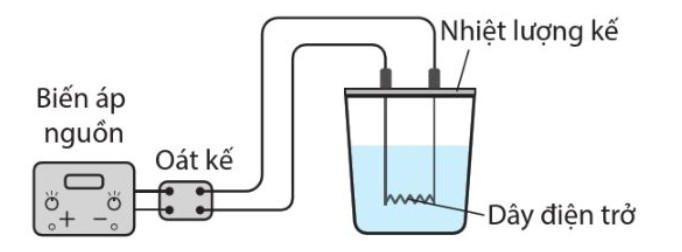
\includegraphics[scale=0.5]{figs/VN12-Y24-PH-SYL-004P-3}}
	\loigiai{\begin{enumerate}[label=\alph*)]
			\item Đúng.
			\item Sai. Oát kế xác định công suất tiêu thụ điện của đoạn mạch.
			\item Đúng.
			\item Đúng.
	\end{enumerate}}
\end{ex}

	% ===================================================================
	\begin{ex}
		\immini{Người ta cọ xát nhiều lần một miếng sắt dẹt có khối lượng \SI{100}{\gram} trên một tấm gỗ. Sau một thời gian thì thấy miếng sắt nóng lên thêm \SI{30}{\celsius}. Cho biết nhiệt dung riêng của sắt là \SI{460}{\joule/\left(\kilogram\cdot\kelvin\right)}.}{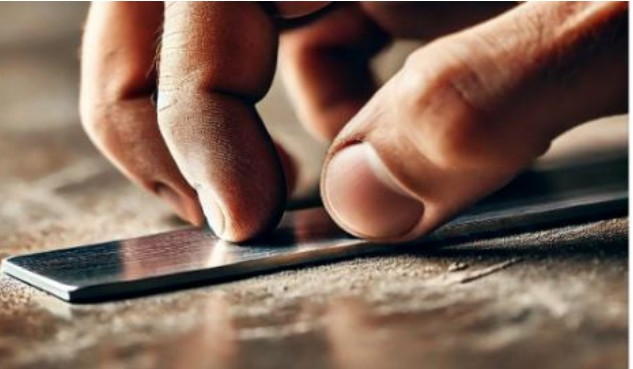
\includegraphics[scale=0.2]{figs/G12Y24B4-3}}
		\choiceTF[t]
		{Trong quá trình cọ xát thì nội năng của miếng sắt giảm}
		{Nội năng của miếng sắt biến thiên là do được truyền nhiệt}
		{Độ biến thiên nội năng của miếng sắt là \SI{1830}{\joule}}
		{Giả sử rằng \SI{60}{\percent} công thực hiện được dùng để làm nóng miếng sắt thì người ta đã tốn một công là \SI{3050}{\joule}}
		\loigiai{}
	\end{ex}
% ===================================================================
\begin{ex}
	Hình 1a biểu diễn sơ đồ của hệ thống làm mát động cơ ô tô. Trong một lần thử nghiệm hệ thống này, các số liệu được thống kê vào Bảng 1b. Coi rằng, khi nhiên liệu bị đốt cháy hoàn toàn thì $\SI{30}{\percent}$ nhiệt năng từ nhiên liệu được chuyển thành cơ năng có ích.
	\begin{center}
		\begin{tabular}{M{7cm}M{10cm}}
			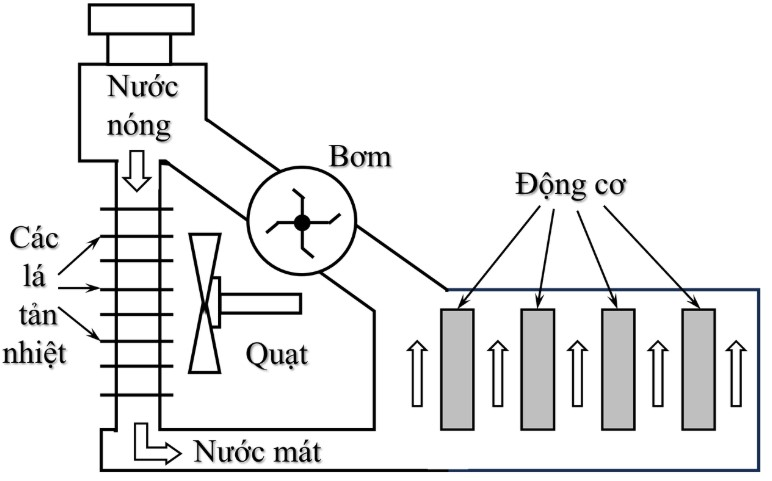
\includegraphics[scale=0.5]{figs/G12Y24B4-1} &\vspace{-0.75cm} \begin{tabular}{|L{8.2cm}|M{1.3cm}|}
				\hline
				Thời gian thử nghiệm (phút) & $\SI{5.0}{}$\\
				\hline
				Khối lượng nhiên liệu tiêu thụ $\left(\si{\kilogram}\right)$ & $\SI{0.80}{}$\\
				\hline
				Năng suất tỏa nhiệt của nhiên liệu $\left(\si{\joule/\kilogram}\right)$ & $\SI{4.6E7}{}$\\
				\hline
				Lưu lượng dòng nước làm mát $\left(\si{\kilogram/\second}\right)$ & $\SI{0.22}{}$\\
				\hline
				Nhiệt độ của nước mát $\left(\si{\celsius}\right)$ & $\SI{30.0}{}$\\
				\hline
				Nhiệt độ của nước nóng $\left(\si{\celsius}\right)$ & $\SI{80.0}{}$\\
				\hline
				Lưu lượng không khí qua các lá tản nhiệt $\left(\si{\kilogram/\second}\right)$ & $\SI{1.25}{}$\\
				\hline
				Nhiệt độ ban đầu của không khí $\left(\si{\celsius}\right)$ & $\SI{20.0}{}$\\
				\hline
				Nhiệt dung riêng của dầu $\left(\si{\joule/\kilogram\cdot\kelvin}\right)$ & $1800$\\
				\hline
				Nhiệt dung riêng của nước $\left(\si{\joule/\kilogram\cdot\kelvin}\right)$ & $4200$\\
				\hline
				Nhiệt dung riêng của không khí $\left(\si{\joule/\kilogram\cdot\kelvin}\right)$ & $760$\\
				\hline
			\end{tabular}\\
			Hình 1a & Bảng 1b
		\end{tabular}
	\end{center}
	
	\choiceTF[t]
	{Có thể thay nước bằng dầu để tăng hiệu quả làm mát động cơ}
	{Nhiệt lượng hao phí trong quá trình thử nghiệm là $\SI{11.04}{\mega\joule}$}
	{\True Nhiệt lượng nước nóng tỏa ra môi trường qua các lá tản nhiệt là $\SI{13.86}{\meter\joule}$}
	{\True Nếu hiệu suất trao đổi nhiệt lượng giữa nước nóng và không khí $\SI{100}{\percent}$ thì nhiệt độ của dòng không khí đi ra khỏi các lá tản nhiệt là $\SI{68.6}{\celsius}$}
	\loigiai{}
\end{ex}
% ===================================================================
\begin{ex}
	Một nhóm học sinh làm thí nghiệm để xác định nhiệt dung riêng của một mẫu kim loại. Họ có một bình xốp hình trụ có vỏ và nắp cách nhiệt, một que khuấy, một nhiệt kế, mẫu kim loại, một chiếc cân và một bình đun nước. Ban đầu, mẫu kim loại được để ở nhiệt độ phòng \SI{27}{\celsius}.
	\begin{center}
		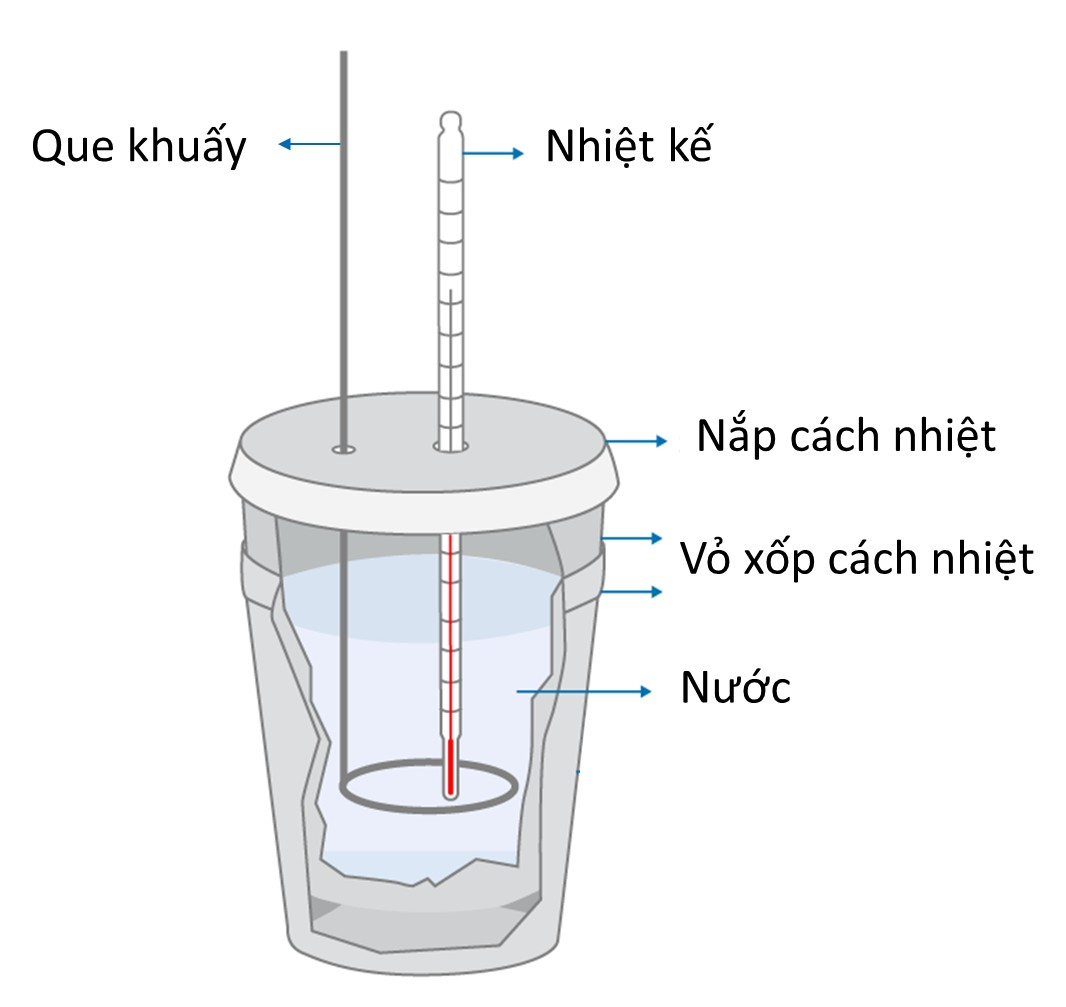
\includegraphics[scale=0.35]{figs/G12Y24B4-2}
	\end{center}
	\choiceTF[t]
	{Nhóm học sinh sử dụng cân và xác định được khối lượng nước đổ vào bình là \SI{0.225}{\kilogram}, khối lượng của mẫu kim loại là \SI{0.409}{\kilogram}. Số chỉ của nhiệt kế nhúng trong nước nóng ngay trước khi thả mẫu kim loại là \SI{67.5}{\celsius} và số chỉ của nhiệt kế khi mẫu kim loại và nước đạt trạng thái cân bằng nhiệt là \SI{56.0}{\celsius}. Biết nhiệt dung riêng của nước là \SI{4180}{\joule/\kilogram\cdot\kelvin}. Từ các số liệu trên, nhóm học sinh xác định được nhiệt dung riêng của mẫu kim loại là \SI{889}{\joule/\kilogram\cdot\kelvin}}
	{\True Nhóm học sinh cho rằng, nếu đun nóng nước tới khoảng \SI{70}{\celsius}, đổ vào bình xốp đã cắm sẵn nhiệt kế, nhẹ nhàng nhúng chìm mẫu kim loại trong nước, đóng kín nắp lại và khuấy nhẹ tay thì số chỉ trên nhiệt kế sau đó sẽ thay đổi liên tục và chỉ dừng lại khi bình xốp chứa nước cùng mẫu kim loại đạt trạng thái cân bằng nhiệt}
	{Nhóm học sinh cho rằng, kết quả tính được ở câu a) nhỏ hơn giá trị nhiệt dung riêng chính xác của mẫu kim loại do trong phép tính đã bỏ qua nhiệt lượng trao đổi với môi trường}
	{Một học sinh trong nhóm cho rằng, nếu bỏ qua thất thoát nhiệt với môi trường thì nhiệt lượng nước thu vào bằng với nhiệt lượng mẫu kim loại tỏa ra}
	\loigiai{}
\end{ex}
\subsection{BÀI TẬP TỰ LUẬN VÀ TRẢ LỜI NGẮN}
\setcounter{ex}{0}
% ===================================================================
\begin{ex}
Thùng nhôm khối lượng $\SI{1.2}{\kilogram}$ đựng $\SI{4}{\kilogram}$ nước ở $\SI{90}{\celsius}$. Cho biết nhiệt dung riêng của nhôm và nước lần lượt là $c_1=\SI{0.92}{\kilo\joule/\kilogram\cdot\kelvin}$, $c_2=\SI{4.186}{\kilo\joule/\left(\kilogram\cdot\kelvin\right)}$. Xác định nhiệt lượng thùng nước toả ra khi nhiệt độ giảm xuống còn $\SI{30}{\celsius}$. Kết quả tính theo đơn vị joule và làm tròn đến chữ số hàng phần mười.
\shortans[oly]{1,07}
	\loigiai{
	Nhiệt lượng do thùng nước toả ra:
	$$Q=\left(m_1c_1+m_2c_2\right)\Delta t=-\SI{1070880}{\joule}.$$
	Vậy nhiệt lượng do thùng nước toả ra là $\SI{1070880}{\joule}$.
	}
	
\end{ex}
% ===================================================================
\begin{ex}
	Để làm nguội nước nóng, người ta trộn $\SI{1.5}{\kilogram}$ nước ở $\SI{25}{\celsius}$ với $\SI{100}{\gram}$ nước ở $\SI{50}{\celsius}$. Xác định nhiệt độ cuối cùng của hỗn hợp khi cân bằng nhiệt. Kết quả làm tròn đến chữ số hàng phần mười.
	\shortans[oly]{26,6}
	\loigiai{
	Khi có sự cân bằng nhiệt, tổng nhiệt lượng trao đổi trong hệ bằng 0:
	$$m_1c\left(t-t_1\right)+m_2c\left(t-t_2\right)=0$$
	$$\Leftrightarrow 1,5\left(t-\SI{25}{\celsius}\right)+0,1\left(t-\SI{50}{\celsius}\right)=0\Rightarrow t=\SI{26.5625}{\celsius}.$$
	}
	
\end{ex}
% ===============================================================
\begin{ex}
	Để xử lí nấm mốc của thóc giống trước khi ngâm, người nông dân dùng nước ấm "nước 3 sôi 2 lạnh" được tạo ra bằng cách trộn 3 phần nước sôi với 2 phần nước lạnh (nước ở nhiệt độ thường). Coi rằng nước lạnh có nhiệt độ là \SI{20}{\celsius}, nước sôi có nhiệt độ \SI{100}{\celsius} và nhiệt tỏa ra xung quanh là không đáng kể. Nhiệt độ của nước sau khi pha là bao nhiêu \si{\celsius}? (Kết quả làm tròn đến hàng đơn vị).
	\shortans[oly]{68}
	\loigiai{
		
	}
\end{ex}
% ===============================================================
\begin{ex}
	Hiện nay, người ta có thể dùng các vỉ đá được làm nóng sẵn trong lò (tăng nội năng của vỉ đá) để nướng thức ăn. Giả sử, một vỉ đá có khối lượng \SI{1.2}{\kilogram}, nhiệt độ ban đầu là \SI{28}{\celsius} được làm nóng trong lò có công suất \SI{20}{\kilo\watt}. Coi như toàn bộ năng lượng của lò cung cấp sẽ dùng để làm nóng vỉ đá. Biết rằng, để làm cho \SI{1}{\kilogram} đá làm vỉ này tăng thêm \SI{1}{\celsius} thì cần nhiệt lượng \SI{5500}{\joule}. Để vỉ đá đạt được nhiệt độ \SI{1000}{\celsius} thì cần thời gian bao nhiêu phút? (Kết quả lấy đến hai chữ số sau dấu phẩy thập phân).
	\shortans[oly]{5,35}
	\loigiai{
		
	}
\end{ex}
% ===============================================================
\begin{ex}
	\immini{Trong một hệ đun nước bằng năng lượng Mặt Trời, năng lượng Mặt Trời thu thập từ những mặt ngoài của phần góp, nó làm cho nước lưu thông qua các ống của phần góp. Bức xạ Mặt Trời đi vào trong phần góp qua các lớp phủ trong suốt, làm nóng nước trong ống. Nước này được bơm vào các bình chứa. Giả thiết rằng hiệu suất của toàn bộ hệ là \SI{20}{\percent} (nghĩa là \SI{80}{\percent} năng lượng Mặt Trời bị mất khỏi hệ). Hỏi diện tích của phần góp là bao nhiêu mét vuông khi cần nâng nhiệt độ của 200 lít nước trong bình chứa từ \SI{20}{\celsius} đến \SI{40}{\celsius} trong 1 giờ. Biết khối lượng riêng của nước là \SI{1000}{\kilogram/\meter^3}; nhiệt dung riêng của nước là \SI{4190}{\joule/\left(\kilogram\cdot\kelvin\right)}; cường độ của ánh sáng Mặt Trời tới là \SI{700}{\watt/\meter^2}. Kết quả làm tròn đến một chữ số sau dấu phẩy thập phân.}{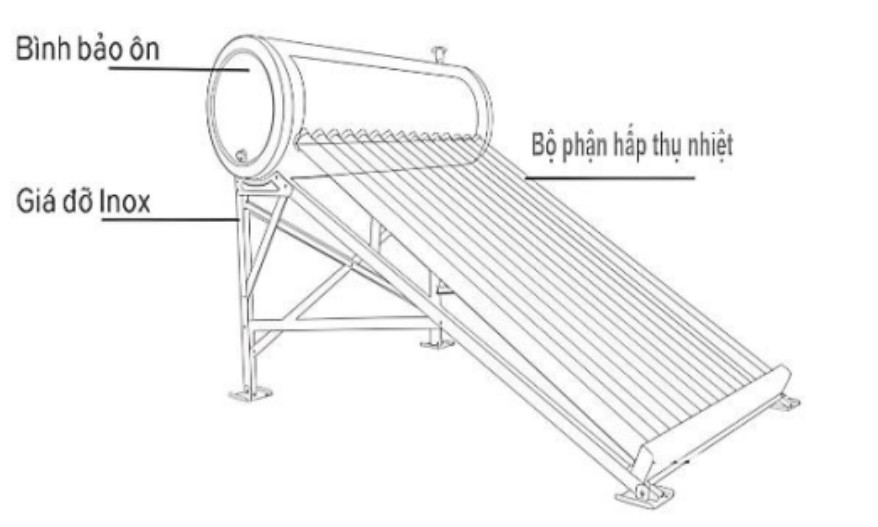
\includegraphics[scale=0.4]{figs/G12Y24B4-4}}
	\shortans[oly]{33,3}
	\loigiai{
		
	}
\end{ex}
% ===================================================================
\begin{ex}
Để xác định nhiệt dung riêng của một chất lỏng, người ta đổ chất lỏng đó vào $\SI{20}{\gram}$ nước ở nhiệt độ $\SI{100}{\celsius}$. Khi có cân bằng nhiệt, nhiệt độ của hỗn hợp đó là $\SI{37.5}{\celsius}$. Khối lượng hỗn hợp là $\SI{140}{\gram}$. Tính nhiệt dung riêng của chất lỏng đó, biết rằng nhiệt độ ban đầu của nó là $\SI{20}{\celsius}$ và hai chất lỏng không tác dụng hoá học với nhau. Cho nhiệt dung riêng của nước $c_2=\SI{4200}{\joule/\left(\kilogram\cdot\kelvin\right)}$. Kết quả tính theo đơn vị $\si{\joule/\left(\kilogram\cdot\kelvin\right)}$.
\shortans[oly]{2500}
	\loigiai{
	Gọi $m$ và $c$ lần lượt là khối lượng và nhiệt dung riêng của chất lỏng cần xác định nhiệt dung riêng.\\
	Khối lượng của chất lỏng đó:
	$$m=m_\text{hh}-m_\text{n}=\SI{120}{\gram}.$$
	Khi hệ đạt trạng thái cân bằng nhiệt thì tổng nhiệt lượng trao đổi của hệ bằng 0:
	$$mc\left(t_\text{cb}-t_0\right)+m_\text{n}c_\text{n}\left(t_\text{cb}-t_\text{0n}\right)=0$$
	$$\Rightarrow c=-\dfrac{m_\text{n}c_\text{n}\left(t_\text{cb}-t_\text{0n}\right)}{m\left(t_\text{cb}-t_0\right)}=\dfrac{\left(\SI{0.02}{\kilogram}\right)\cdot\left[\SI{4200}{\joule/\left(\kilogram\cdot\kelvin\right)}\right]\cdot\left(\SI{37.5}{\celsius}-\SI{100}{\celsius}\right)}{\left(\SI{0.12}{\kilogram}\right)\cdot\left(\SI{37.5}{\celsius}-\SI{20}{\celsius}\right)}=\SI{2500}{\joule/\left(\kilogram\cdot\kelvin\right)}.$$
	}
	
\end{ex}
% ===================================================================
\begin{ex}
	Để xác định nhiệt độ của một chiếc lò, người ta đốt nóng trong lò một cục sắt khối lượng $m_1=\SI{0.5}{\kilogram}$ rồi thả nhanh vào trong bình chứa $m_2=\SI{4}{\kilogram}$ nước có nhiệt độ ban đầu là $\SI{18}{\celsius}$. Nhiệt độ cuối cùng trong bình là $\SI{28}{\celsius}$. Hãy xác định nhiệt độ của lò theo đơn vị \si{\celsius}. Bỏ qua trao đổi nhiệt với vỏ bình và quá trình nước hoá hơi khi tiếp xúc với cục sắt nóng. Cho nhiệt dung riêng của sắt là $c_1=\SI{460}{\joule/\left(\kilogram\cdot\kelvin\right)}$, nhiệt dung riêng của nước là $c_2=\SI{4200}{\joule/\left(\kilogram\cdot\kelvin\right)}$. Kết quả làm tròn đến chữ số hàng đơn vị.
	\shortans[oly]{758}
	\loigiai{
	Khi cân bằng nhiệt, tổng nhiệt lượng trao đổi trong hệ bằng 0:
	$$m_1c_1\left(t_\text{cb}-t_1\right)+m_2c_2\left(t_\text{cb}-t_2\right)=0\Rightarrow t_1\approx\SI{758.4}{\celsius}.$$
	}
	
\end{ex}

% ===================================================================
\begin{ex}
Người ta đổ $m_1 =\SI{200}{\gram}$ nước sôi có nhiệt độ $t_1 =\SI{100}{\celsius}$ vào một chiếc cốc có khối lượng $m_2 = \SI{120}{\gram}$ đang ở nhiệt độ $t_2 =\SI{20}{\celsius}$. Sau khoảng thời gian $T = \SI{5}{\text{phút}}$, nhiệt độ của cốc nước bằng $t=\SI{40}{\celsius}$. Xem rằng sự mất nhiệt xảy ra một cách điều đặn, hãy xác định nhiệt lượng tỏa ra môi trường xung quanh trong mỗi giây. Cho nhiệt dung riêng nước và thuỷ tinh lần lượt là $c_1=\SI{4200}{\joule/\left(\kilogram\cdot\kelvin\right)}$, $c_2=\SI{840}{\joule/\left(\kilogram\cdot\kelvin\right)}$. Kết quả tính theo đơn vị \si{\joule/\second} và làm tròn đến chữ số hàng đơn vị.
\shortans[oly]{161}
	\loigiai{Nhiệt lượng nước sôi toả ra để giảm nhiệt độ từ $\SI{100}{\celsius}$ còn $\SI{40}{\celsius}$:
		$$Q_\text{toả}=m_1c_1\left(t_1-t\right)=\SI{50400}{\joule}.$$
		Nhiệt lượng cốc thuỷ tinh thu vào để tăng nhiệt độ từ $\SI{20}{\celsius}$ lên $\SI{40}{\celsius}$:
		$$Q_\text{thu}=m_2c_2\left(t-t_2\right)=\SI{2016}{\joule}.$$
		Nhiệt lượng toả ra môi trường trong mỗi giây:
		$$w=\dfrac{Q_\text{toả}-Q_\text{thu}}{T}=\SI{161.28}{\joule/\second}.$$
	}
	
\end{ex}
% ===================================================================
\begin{ex}
	Trộn ba chất lỏng không tác dụng hoá học với nhau có khối lượng lần lượt là $m_1=\SI{2}{\kilogram}$, $m_2=\SI{3}{\kilogram}$, $m_3=\SI{4}{\kilogram}$. Biết nhiệt dung riêng và nhiệt độ ban đầu của mỗi chất lỏng lần lượt là $c_1=\SI{2000}{\joule/\left(\kilogram\cdot\kelvin\right)}$, $t_1=\SI{57}{\celsius}$, $c_2=\SI{4000}{\joule/\left(\kilogram\cdot\kelvin\right)}$, $t_2=\SI{63}{\celsius}$, $c_3=\SI{3000}{\joule/\left(\kilogram\cdot\kelvin\right)}$, $t_3=\SI{92}{\celsius}$. Nhiệt độ của hỗn hợp khi cân bằng nhiệt là bao nhiêu \si{\celsius}? Kết quả làm tròn đến chữ số hàng phần mười.
	\shortans[oly]{74,6}
	\loigiai{Khi cân bằng nhiệt, tổng nhiệt lượng trao đổi trong hệ bằng 0:
		$$m_1c_1\left(t_\text{cb}-t_1\right)+m_2c_2\left(t_\text{cb}-t_2\right)+m_3c_3\left(t_\text{cb}-t_3\right)=0$$
		$$\Rightarrow t_\text{cb}=\dfrac{m_1c_1t_1+m_2c_2t_2+m_3c_3t_3}{m_1c_1+m_2c_2+m_3c_3}\approx\SI{74.6}{\celsius}.$$
	}
	
\end{ex}
 %===================================================================
\begin{ex}
	Một khối sắt có khối lượng $m$ ở nhiệt độ $\SI{150}{\celsius}$ khi thả vào một bình nước thì làm nhiệt độ nước tăng từ $\SI{20}{\celsius}$ lên $\SI{60}{\celsius}$. Thả tiếp vào nước khối sắt thứ hai có khối lượng $\dfrac{m}{2}$ ở $\SI{100}{\celsius}$ thì nhiệt độ sau cùng của nước là bao nhiêu \si{\celsius}? Coi như chỉ có sự trao đổi nhiệt giữa khối sắt với nước và bỏ qua quá trình nước hoá thành hơi khi tiếp xúc với sắt nóng. Kết quả làm tròn đến chữ số hàng phần mười.
	\shortans[oly]{65,3}
	\loigiai{	Gọi:
		\begin{itemize}
			\item $m_2$ là khối lượng nước trong bình;
			\item $c_1$, $c_2$ lần lượt là nhiệt dung riêng của sắt và nước;
			\item $t_1$, $t_2$ lần lượt là nhiệt độ ban đầu của thỏi sắt khối lượng $m$ và nước.
		\end{itemize}
		\textbf{Bỏ khối sắt khối lượng $m$ vào nước}\\
		Khi có cân bằng nhiệt, nhiệt lượng trao đổi trong hệ bằng 0:
		$$mc_1\left(t_\text{cb}-t_1\right)+m_2c_2\left(t_\text{cb}-t_2\right)=0\Rightarrow \dfrac{mc_1}{m_2c_2}=\dfrac{t_\text{cb}-t_2}{t_1-t_\text{cb}}=\dfrac{4}{9}.$$
		\textbf{Bỏ thêm khối sắt khối lượng $m/2$ vào nước}\\
		Khi có cân bằng nhiệt, nhiệt lượng trao đổi trong hệ bằng 0:
		$$\left(mc_1+m_2c_2\right)\left(t'_\text{cb}-t_\text{cb}\right)+\dfrac{m}{2}c_1\left(t'_\text{cb}-t'_1\right)=0$$
		$$\Rightarrow \Rightarrow t'_\text{cb}=\dfrac{mc_1\left(t_\text{cb}+\dfrac{t'_1}{2}\right)+m_2c_2t_\text{cb}}{1,5mc_1+m_2c_2}=\dfrac{\dfrac{4}{9}\cdot\left(\SI{60}{\celsius}+\SI{50}{\celsius}\right)+\SI{60}{\celsius}}{1,5\cdot\dfrac{4}{9}+1}\approx\SI{65.33}{\celsius}.$$
	}
	
\end{ex}
%% ===================================================================
%\begin{ex}
%Có hai bình cách nhiệt. Bình 1 chứa $m_1 =\SI{2}{\kilogram}$ nước ở $t_1=\SI{20}{\celsius}$, bình 2 chứa $m_2 =\SI{4}{\kilogram}$ nước ở $t_2 =\SI{60}{\celsius}$. Người ta rót một lượng nước $m$ từ bình 1 sang bình 2, sau khi cân bằng nhiệt, người ta lại rót một lượng nước từ bình 2 sang bình 1. Nhiệt độ cân bằng ở bình 1 lúc này là $\SI{21.95}{\celsius}$.
%\begin{enumerate}[label=\alph*)]
%	\item Tính lượng nước $m$ rong mỗi lần rót và nhiệt độ cân bằng ở bình 2.
%	\item Nếu tiếp tục thực hiện lần hai, tìm nhiệt độ cân bằng ở mỗi bình.
%\end{enumerate}
%	\loigiai{\begin{enumerate}[label=\alph*)]
%			\item \begin{itemize}
%				\item \textbf{Rót nước từ bình 1 sang bình 2}\\
%				Khi cân bằng nhiệt, tổng nhiệt lượng trao đổi của $m$ và lượng nước ở bình 2 bằng 0:
%				$$mc\left(t'_2-t_1\right)+m_2c\left(t'_2-t_2\right)=0$$
%				\begin{equation}
%					\label{eq:4P-5}
%					m\left(t'_2-t_1\right)=m_2\left(t_2-t'_2\right)
%				\end{equation}
%				\item \textbf{Rót nước từ bình 2 sang bình 1}\\
%				Khi cân bằng nhiệt, tổng nhiệt lượng trao đổi của $m$ và lượng nước ở bình 1 bằng 0:
%				$$mc\left(t'_1-t\right)+\left(m_1-m\right)c\left(t'_1-t_1\right)=0$$
%				\begin{equation}
%					\label{eq:4P-6}
%					m\left(t-t_1\right)=m_1\left(t'_1-t_1\right)
%				\end{equation}
%				Từ (\ref{eq:4P-5}) và (\ref{eq:4P-6}), suy ra:
%				\begin{equation*}
%					\begin{cases}
%						t=\dfrac{m_2t_2-m_1\left(t'_1-t_1\right)}{m_2}\approx\SI{59}{\celsius}\\
%						m=\dfrac{m_1m_2\left(t'_1-t_1\right)}{m_2\left(t_2-t_1\right)-m_1\left(t'_1-t_1\right)}\approx\SI{0.1}{\kilogram}
%					\end{cases}
%					.
%				\end{equation*}
%			\end{itemize}
%			\item Thực hiện lần hai, nhiệt độ cân bằng của mỗi bình là
%			$$t''_2=\dfrac{mt'_1+m_2t'_2}{m+m_2}=\SI{58.12}{\celsius};\quad t''_1=\dfrac{mt''_2+\left(m_1-m\right)t_1}{m_1}=\SI{23.76}{\celsius}.$$
%		\end{enumerate}
%	}
%	
%\end{ex}
% ===================================================================
\begin{ex}
	Trộn lẫn rượu vào nước, người ta thu được một hỗn hợp nặng $\SI{120.8}{\gram}$ ở nhiệt độ $\SI{30}{\celsius}$. Tính khối lượng nước và rượu đã pha, biết rằng ban đầu rượu ở nhiệt độ $\SI{10}{\celsius}$ và nước ở nhiệt độ $\SI{90}{\celsius}$. Cho nhiệt dung riêng của rượu và nước lần lượt là $\SI{2500}{\joule/\left(\kilogram\cdot\kelvin\right)}$, $\SI{4200}{\joule/\left(\kilogram\cdot\kelvin\right)}$.
	\loigiai{
		Gọi:
		\begin{itemize}
			\item $m_1, c_1, t_1$ lần lượt là khối lượng, nhiệt dung riêng và nhiệt độ ban đầu của rượu;
			\item $m_2, c_2, t_2$ lần lượt là khối lượng, nhiệt dung riêng và nhiệt độ ban đầu của nước.
		\end{itemize}
		Ta có:
		\begin{equation}
			\label{eq:4P-1}
			m_1+m_2=\SI{120.8}{\gram}=\SI{0.1208}{\kilogram}
		\end{equation}
		Khi hệ cân bằng nhiệt, tổng nhiệt lượng trao đổi trong hệ bằng 0:
		$$m_1c_1\left(t_\text{cb}-t_1\right)+m_2c_2\left(t_\text{cb}-t_2\right)=0$$
		\begin{equation}
			\label{eq:4P-2}
			50000m_1-252000m_2=0
		\end{equation}
		Từ (\ref{eq:4P-1}) và (\ref{eq:4P-2}) suy ra:
		\begin{equation*}
			\begin{cases}
				m_1=\SI{100.8}{\gram}\\
				m_2=\SI{20}{\gram}
			\end{cases}
			.
		\end{equation*}
	}
	
\end{ex}
% ===================================================================
\begin{ex}
	Bỏ một vật rắn khối lượng $\SI{100}{\gram}$ ở $\SI{100}{\celsius}$ vào $\SI{500}{\gram}$ nước ở $\SI{15}{\celsius}$ thì nhiệt độ sau cùng của vật là $\SI{16}{\celsius}$. Thay nước bằng $\SI{800}{\gram}$ chất lỏng khác ở $\SI{10}{\celsius}$ thì nhiệt độ sau cùng là $\SI{13}{\celsius}$. Tìm nhiệt dung riêng của vật rắn và chất lỏng. Cho nhiệt dung riêng của nước là $c = \SI{4200}{\joule/\left(\kilogram\cdot\kelvin\right)}$.
	\loigiai{
		\textbf{Khi bỏ vật rắn vào nước:}\\
		Khi cân bằng nhiệt, tổng nhiệt lượng trao đổi của vật rắn và nước bằng 0:
		$$m_vc_v\left(t_\text{cb}-t_v\right)+m_nc_n\left(t_\text{cb}-t_n\right)=0\Rightarrow c_v=\dfrac{m_nc_n\left(t_\text{cb}-t_n\right)}{m_v\left(t_v-t_\text{cb}\right)}=\SI{250}{\joule/\left(\kilogram\cdot\kelvin\right)}.$$
		\textbf{Khi bỏ vật rắn vào trong chất lỏng khác}\\
		Khi cân bằng nhiệt, tổng nhiệt lượng trao đổi của vật rắn và chất lỏng bằng 0:
		$$m_vc_v\left(t'_\text{cb}-t_v\right)+m_lc_l\left(t'_\text{cb}-t_l\right)\Rightarrow c_l=\dfrac{m_vc_v\left(t_v-t_\text{cb}\right)}{m_l\left(t'_\text{cb}-t_l\right)}=\SI{906.25}{\joule/\left(\kilogram\cdot\kelvin\right)}.$$
	}
	
\end{ex}